\documentclass{beamer}
\usepackage{subfig}
\usepackage{amsmath}
\usepackage{bm}
\usepackage[T1]{fontenc}

\DeclareMathOperator*{\argmax}{arg\,max}
\DeclareMathOperator*{\argmin}{arg\,min}


\title{Model Predictive Control}
\author{Prof. Alessandro Lucantonio}
\institute{Aarhus University}
\date{}

\setbeamertemplate{footline}[frame number]
\setbeamertemplate{navigation symbols}{}


\begin{document}
	\frame{\titlepage}
	
	
			
			\begin{frame}
				\frametitle{Model Predictive Control - Main features}
				MPC uses a \textbf{model} of the system to \textbf{predict} future states $x_i \in \mathbb{R}^n$, $i=0,\dots,N-1$ and optimize \textbf{control} inputs $u_i \in \mathbb{R}^m$, $i=0,\dots,M-1$ over a defined \textit{time horizon}.
				
				\vspace{5mm}
				
				Key components:
				\begin{itemize}
				\item \textbf{Predictive Model}: Represents the dynamics of the system (linear/non-linear, discrete/continuous).
				\item \textbf{Horizon}: Consists of a prediction horizon ($N$ future time-steps) and a control horizon ($M$ future time-steps).
				\item \textbf{Cost function}: Defined to quantify the desired system performance, typically involves minimizing \textit{error} (of system trajectory with respect to desired/\textit{setpoint} $\bar{x}_i$) and \textit{control effort} (here $N=M$):
				$$ J = \sum_{i=0}^{N-1}[{s\|x_i - \bar{x}_i\|^2} + q\|u_i\|^2]$$
				with $s$ and $q$ weights of the cost function terms.
				\end{itemize}
		
				
			\end{frame}
			
		\begin{frame}
				\frametitle{Model Predictive Control - Algorithm}
				
			\begin{columns} 
				% Column 1
				\begin{column}{.52\textwidth}
					%Basic steps:
					\begin{enumerate}
						\item Choose an initial sequence of controls;
						\item Measure current state of the system;
						\item Predict future states $x_i$ using the model, upon applying a sequence of controls $u_i$;
						\item Solve an optimization problem to minimize the cost function $J$ with respect to the controls $u_i$, subject to constraints (such as bounds on the controls).
						\item Apply $u_0$ and go to step 2.
					\end{enumerate}
					%\vspace{5mm}
					%We can use a \textbf{genetic algorithm} to solve the optimization problem.
				\end{column}
				% Column 2    
				\begin{column}{.52\textwidth}
					\begin{figure}
						\centering
						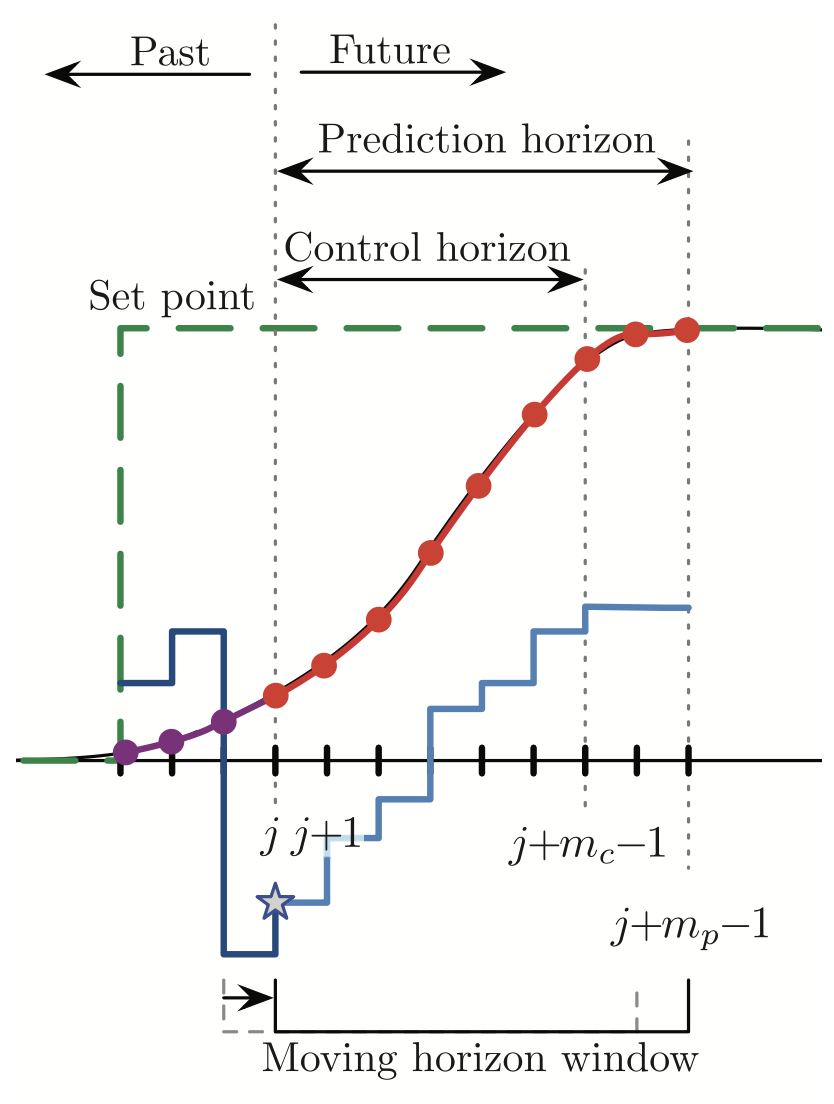
\includegraphics[scale=0.35]{images/mpc_intro}
						%\caption{}
						\label{fig:mpcintro}
					\end{figure}
				\end{column}
				
			\end{columns}
				
			
			
			
			
		\end{frame}
	
\end{document}